\section{Overview of the pseudonymization procedure}
PseudoID has a number of assumption about the underlying experimental procedures. These assumptions were defined so that they should be easy to fit to the majority of medical research experiments. The pseudonymization workflow of SFB289 is illustrated on Fig. \ref{fig:flowchart} and includes the following steps.

\begin{figure}[H]
\centering
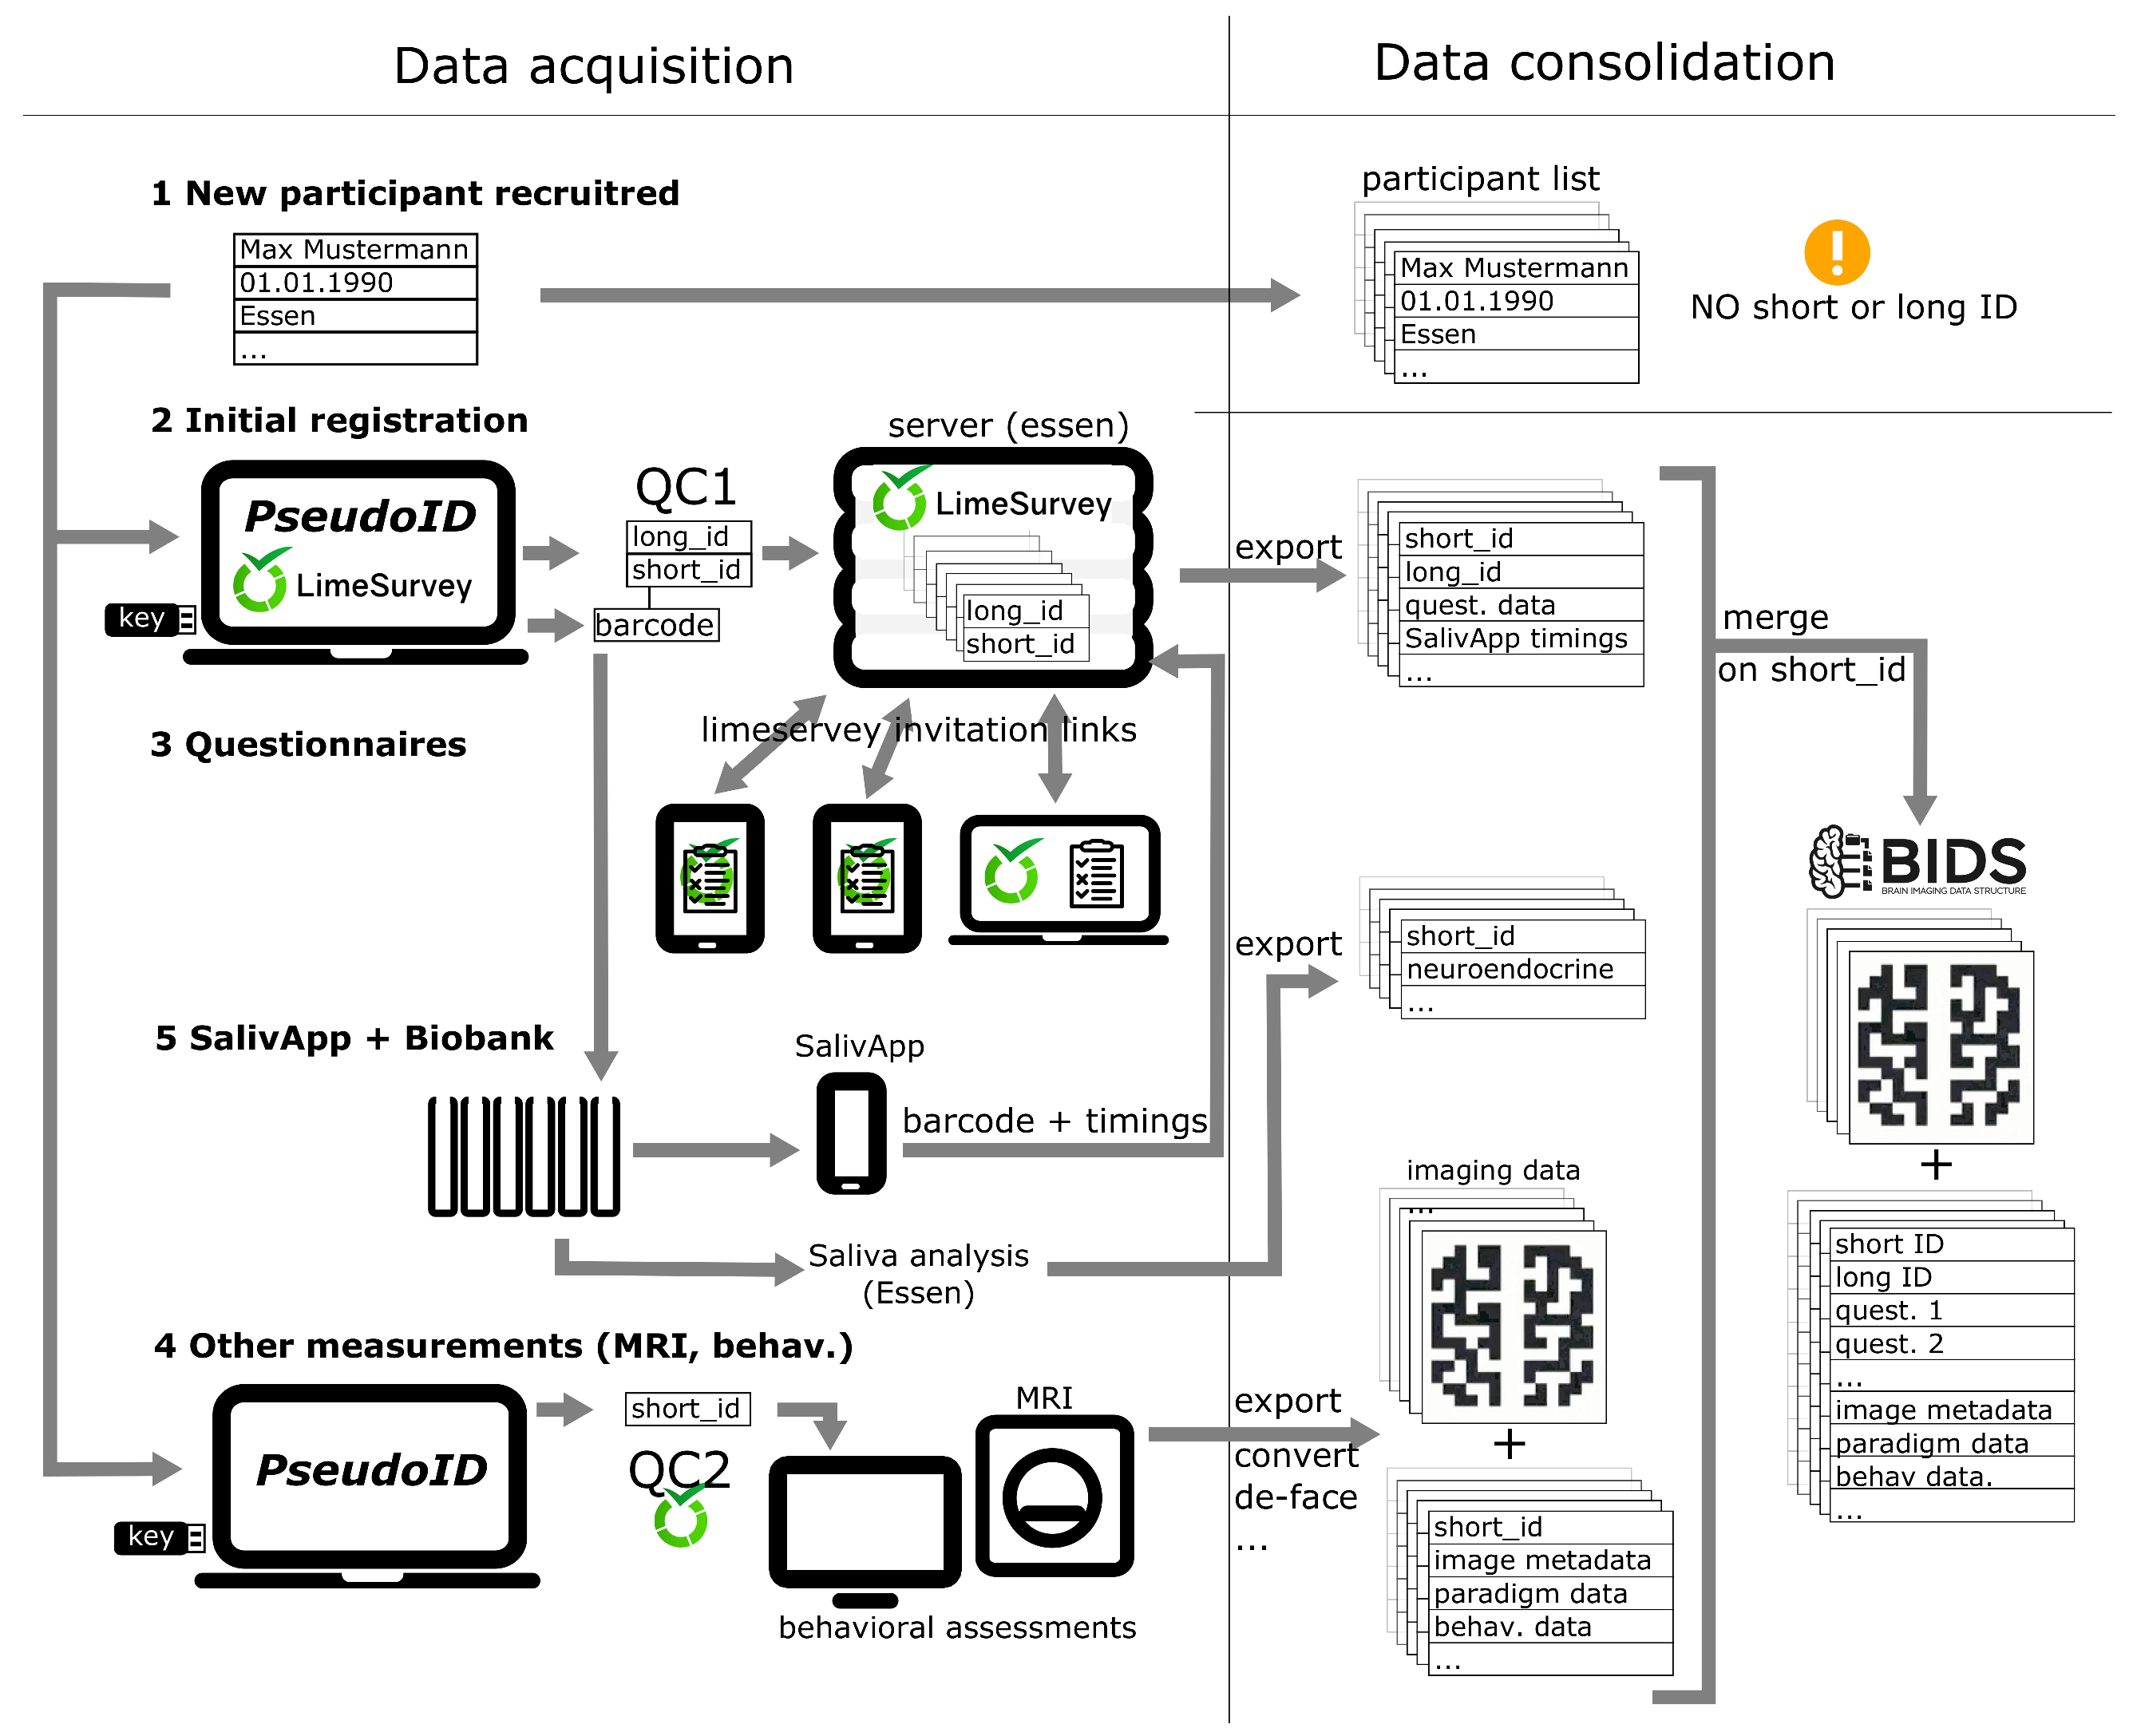
\includegraphics[width=1.0\textwidth]{docs/fig/overview_v2.eps}
\caption{The pseudonymization workflow of SFB289}
\label{fig:flowchart}
\end{figure}

\InsertBoxR{1}{
\small\setlength\fboxsep{5pt}\setlength\fboxrule{1pt}
\fcolorbox{pniblue}{pniblue!5}{\begin{minipage}{0.5\textwidth}
Important Note: the pseudonyms must never be stored in the participant list!
\end{minipage}}
}[1]

\par\noindent\rule{\textwidth\color{pniblue}}{0.4pt}
\textbf{1. Participant recruitment:}
When a new participant is recruited, his/her personal data and availability (e.g. phone number, e-mail) is recorded on-site (e.g. during a telephone interview). These data is saved into a "participant list" (responsibility of the single projects). While this participant list itself is also to be protected, PseudoID is not reliable for the protection of this data. In fact, the main goal of PseudoID is to make it impossible to link this data to the experimental datasets (unless owning the pseudonymization secret).
%%\par\noindent\rule{\textwidth\color{pniblue}}{0.4pt}
%\InsertBoxR{-1}{
%\small\setlength\fboxsep{5pt}\setlength\fboxrule{1pt}
%\fcolorbox{pniblue}{pniblue!5}{\begin{minipage}{0.45\textwidth}
%Importantly, even though the web browser is used as a user interface for the software %(thus it looks like a webpage), personal data always stays on the local computer hosting %the software and hardware key.
%\end{minipage}}
%}[1]

\vspace{1}

\par\noindent\rule{\textwidth\color{pniblue}}{0.4pt}
\textbf{2. Initial registration:} The dedicated hardware key (provided by Z03) is connected to an experimental computer via the USB port. As a next step, the following personal data is entered into PseudoID, through its browser interface (depicted on the left of Fig. \ref{fig:screenshots}): first and last name, date of birth, place of birth, mother's surname.

Importantly, even though the web browser is used as a user interface for the software (thus it looks like a webpage), \textbf{personal data always stays on the local computer} hosting the software and hardware key.


\begin{figure}
%\centering
\subfigure{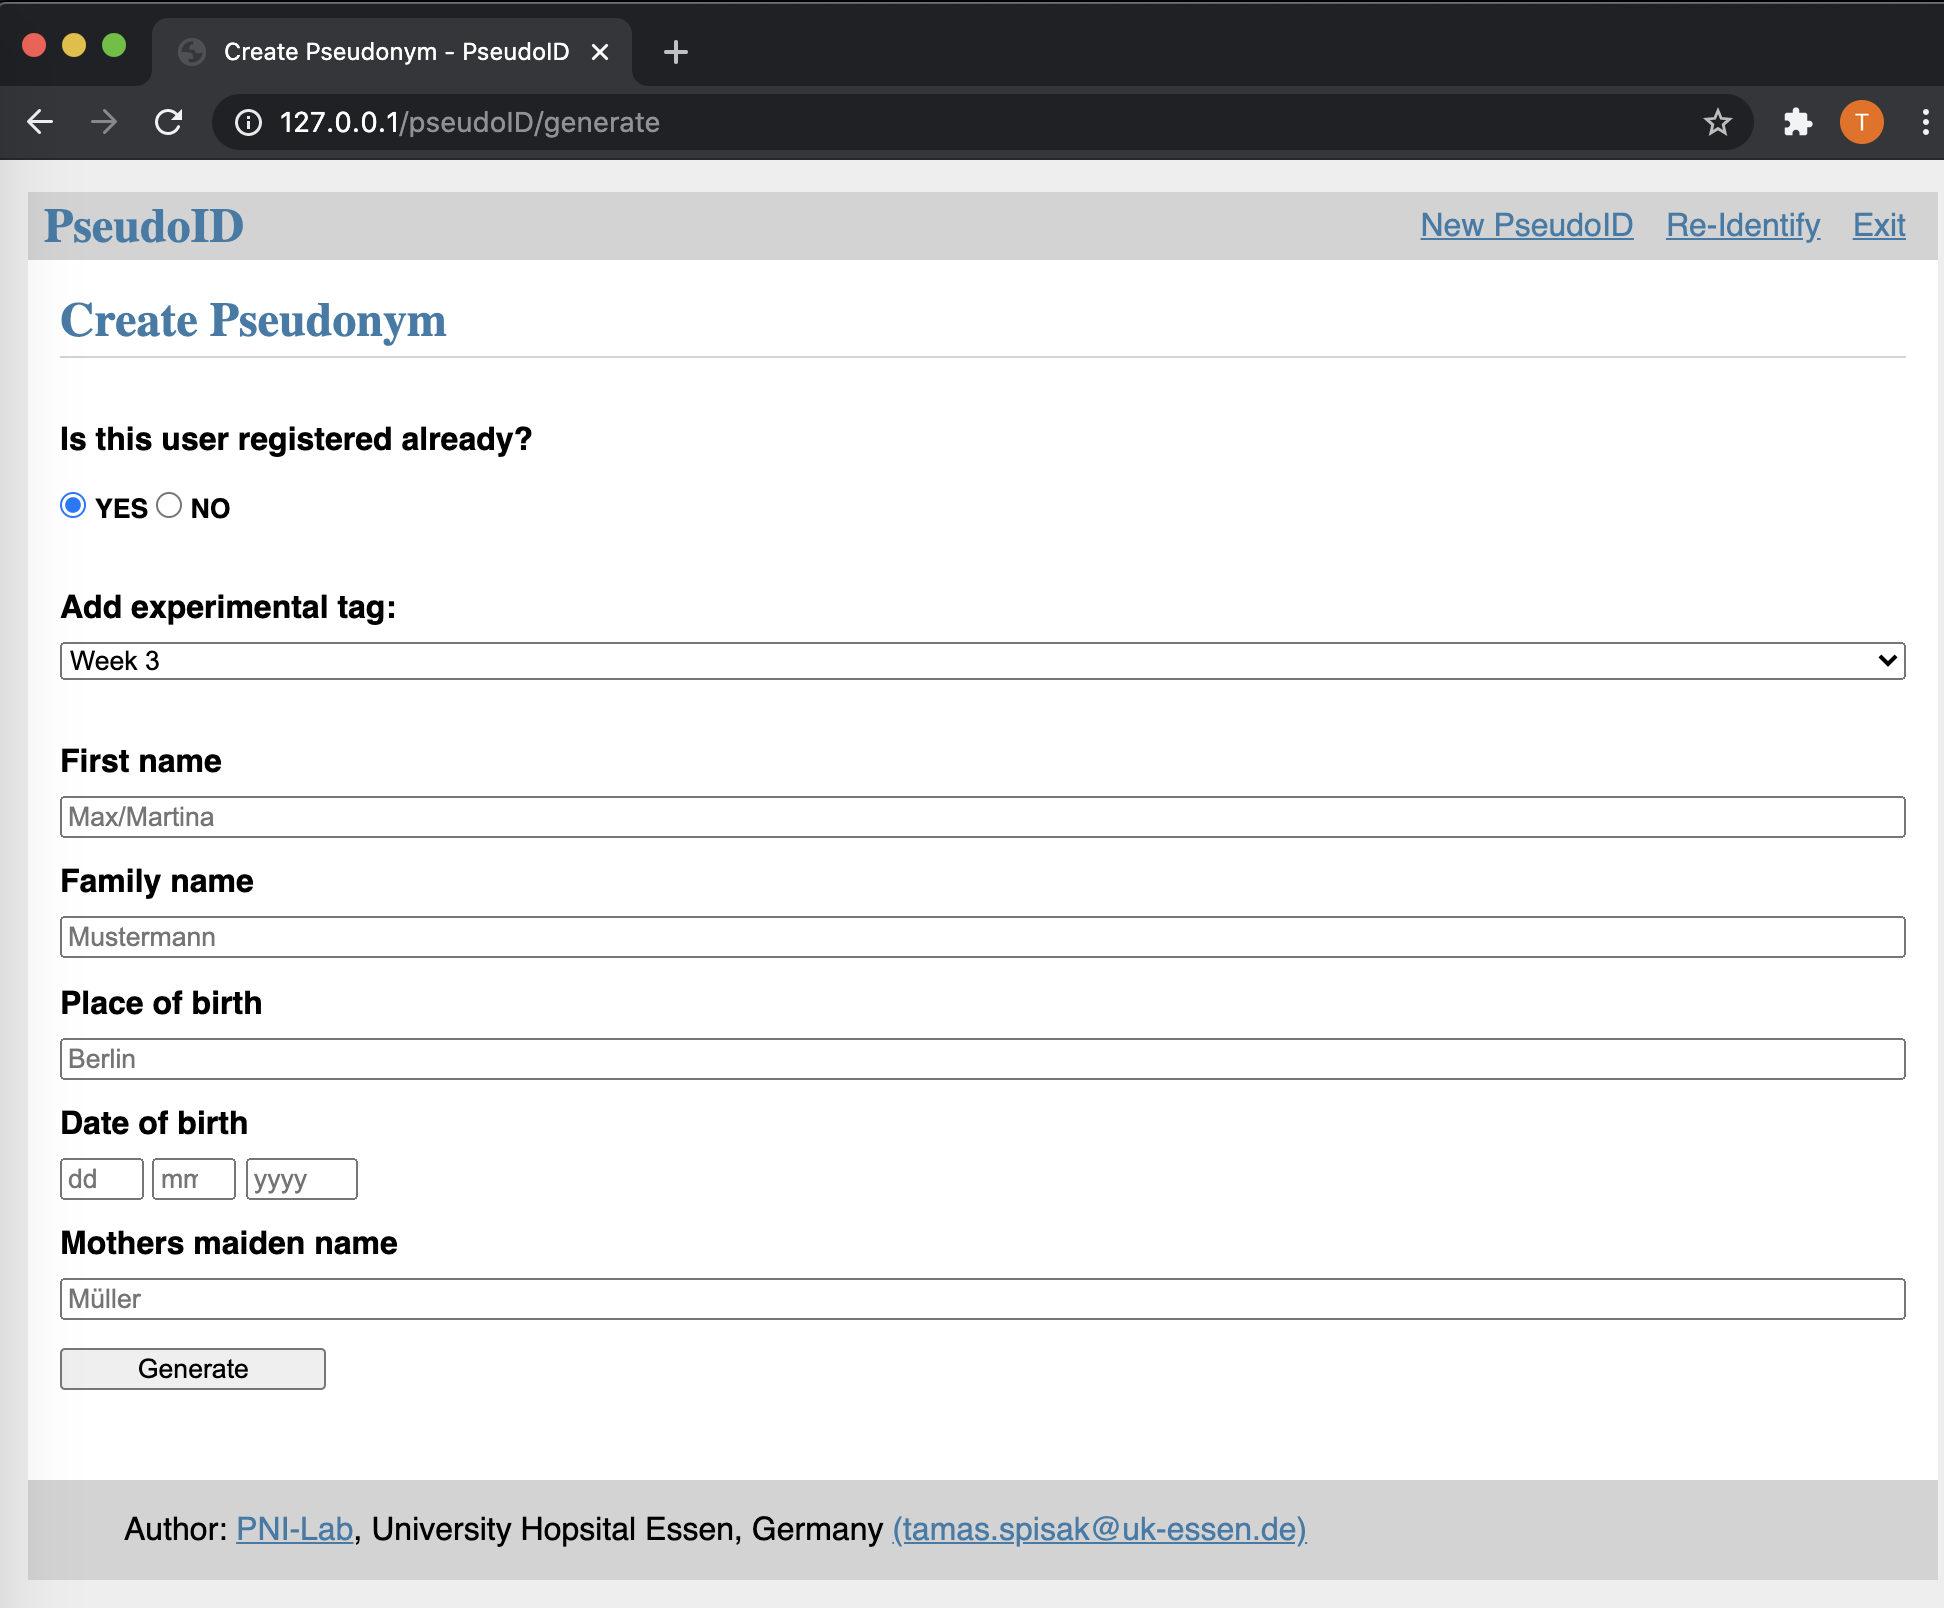
\includegraphics[width=.45\textwidth]{docs/fig/pseudoID_generate.png}}
\hfill
\subfigure{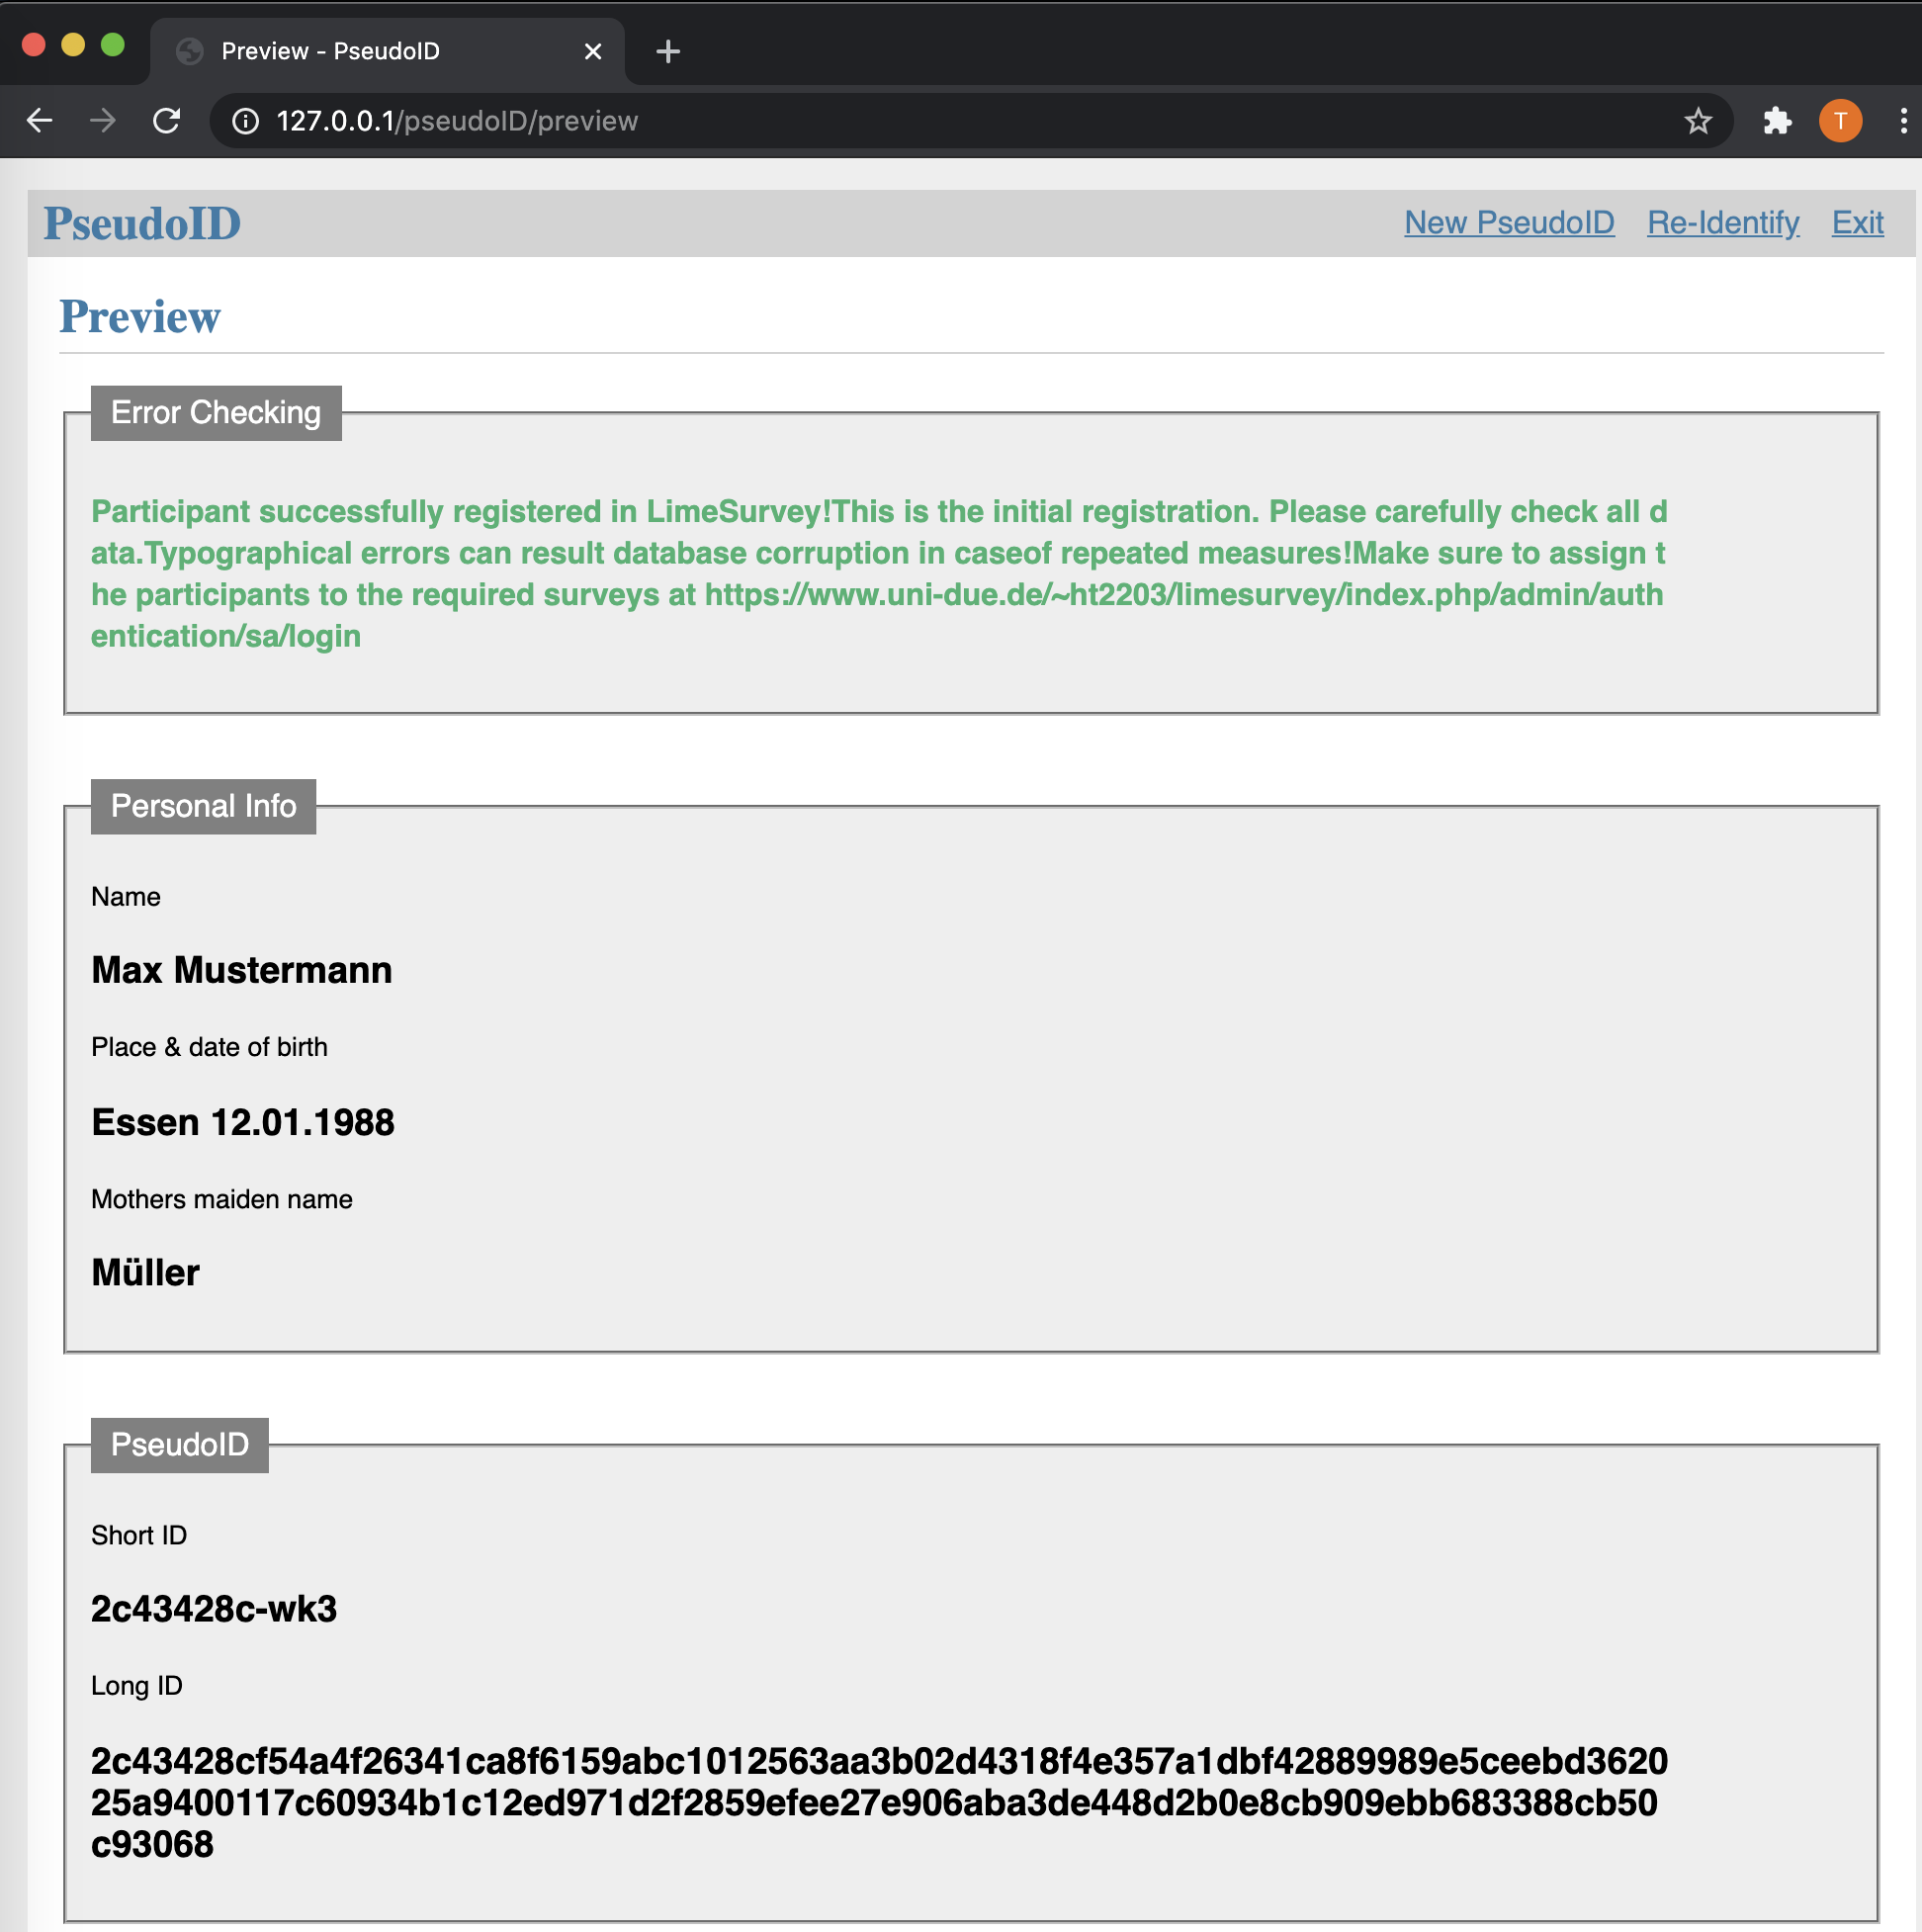
\includegraphics[width=.45\textwidth]{docs/fig/pseudoID_preview.png}}
\caption{The browser-based user interface of PseudoID.}
\label{fig:screenshots}
\end{figure}

PseudoID reads the "pseudonymization secret" from the hardware key and uses it to generate pseudonym. After the user confirms that the data is correct, the software outputs the long and short-version of the pseudonym (on the right of Fig. \ref{fig:screenshots}). Both the long and short IDs are unique for the whole CRC. De-identification is only possible with the long-id. During the initial registration, PseudoID automatically connects to the LimeSurvey server hosted at the University Duisburg-Essen and registers the participant's long and short IDs in the central participant database. Additionally, PseudoID converts the short ID into a barcode (see step 5).

\par\noindent\rule{\textwidth\color{pniblue}}{0.4pt}
\textbf{3. Questionnaires:}
 Questionnaire data will be collected with LimeSurvey. After the researcher has assigned a participant from the central participant database to a questionnaire, the participant can be invited to the questionnaire with a link and a dedicated accession code. Questionnaires can be filled in on any computer (or tablet), with internet connection. 
 If the initial registration and the assignment of the participant to a given questionnaire take place in different time points (e.g repeated measures), PseudoID can be used again to obtain the short ID of the participant, given his/her personal data (either from local 'participant list' or as provided by the participant.
 Multiple assessment points (repeated measures) are natively supported by LimeSurvey.
 
 \par\noindent\rule{\textwidth\color{pniblue}}{0.4pt}
 \textbf{4. Other measurements (MRI, behavior):}
 For other measurements, PseudoID can be used again to obtain the shortID of the participant (given the hardware key). The short ID can than be used in the dedicated experimental system (e.g. the MRI console) as the identifier ("name") of the participant, so that it gets exported together with the experimental data. In case of repeated measurements, PseudoID can be used again and again to obtain the short ID. For convenience, it is also possible to assign standard "experimental tags" to the short ID (e.g. -w2 for week 2)

\par\noindent\rule{\textwidth\color{pniblue}}{0.4pt} 
\textbf{5. Compatibility with SalivApp, genetic assessment and Biobank:} Upon the initial registration, PseudoID generates a barcode for the short ID. These can be printed by the barcode printers provided by the central projects and used to label the saliva sampling kit for the given participant. This barcode-labels will be scanned by the smartphone application (SalivApp) during sample collection (for precise timing) and the BioBank during analysis.

\par\noindent\rule{\textwidth\color{pniblue}}{0.4pt}
\textbf{Data Consolidation and re-identification):} The experimental data (either exported form the LimeSurvey Database, or via the dedicated experimental systems) - if required - will be subject of further anonymization (e.g. de-facing of structural MRI images) with software provided by the central scientific project. Merging of experimental data from different sources or different assessment points is based on the short ID. The LimeSurvey database provides the link between the short and long IDs. The latter can be used for re-identification, e.g. in case of incidental findings by the owners of the hardware key.
